\subsection{Single Transistor Circuits}
MOSFETS are cool. They really have multiple modes of function with their different "regimes", which allow them to preform several functions. One thing to keep in mind, as a rule of thumb, circuits are always drawn in a way to have the higher potential on top and the lowest potential on the bottom of the circuit. So you'll pretty much always see ground at the bottom and $V_dd$ at the top, hopefully this will help you read through the circuits more easily. 
\subsubsection{The Current Source}
The simplest function of a MOSFET, it is obtained by holding source and gate voltage at constant values. As long as the difference between the drain and source voltages is larger than approximately $4U_T$, the nFET in \textbf{saturation and subthreshold} reduces to:
\begin{equation}
    I_{ds} =  I_{n0} e^{\frac{\kappa_{n}V_g - V_s}{U_T}}
\end{equation}
Remember from our interlude that this is a First-Order approximation (i.e., it neglects Second-Order effects such as the Early Effect). This basically yields the assumption that the drain current is independent of the drain voltage. The The above threshold equation is derived in the textbook and out of the scope of these lecture notes - though one should remember that it is different than this one! It also happens that the Early Effect makes current source more ideal than when operating above threshold. 
Note that most often, current source encountered in circuits are pFETs rather.

\begin{figure}[H]
    \centering
    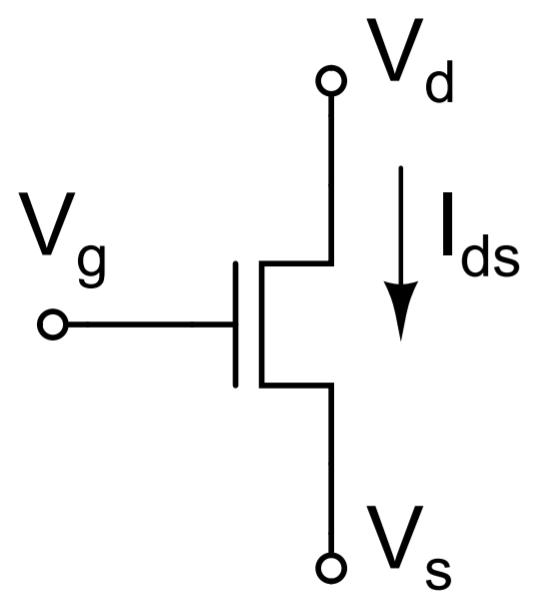
\includegraphics[width=0.25\linewidth]{../../Figures/N_FET_Current_Source.PNG}
    \caption{nFET Current Source. Adapted from Lecture Notes.}
    \label{fig:basalandcerebellum}
\end{figure}

\subsubsection{Linear Resistor}

With some calculation and a lot of approximation, we manage to reach Ohm's relation, back from the known $I_{ds}$ equation. This means we have an independent quantity that links between voltage and current: resistance.  

\begin{equation}
I_{ds} = I_{n0} e^{\frac{\kappa_{n}V_g}{U_T}}(e^\frac{-V_s}{U_T} - e^\frac{-V_d}{U_T})
\end{equation}
With some rearranging, we get: 
\begin{equation}
I_{ds} = I_{n0} e^{(\frac{\kappa_n V_g}{U_T}-\frac{V_d + V_s}{2U_T})}(e^{\frac{V_d - V_s}{2U_T}} - e^{-\frac{-(V_d - V_s)}{2U_T}})
\end{equation}
Lucky us, the second term looks like a sinh! (Remember: $sinh(x) = \frac{e^x - e^{-x}}{2}$). 
We thus reach: 
\begin{equation}
I_{ds} = 2I_{n0} e^{(\frac{\kappa_n V_g}{U_T}-\frac{V_d + V_s}{2U_T})}sinh(\frac{V_d - V_s}{2U_T})
\end{equation}
And here comes the approximation that will please mathematicians: If $V_d - V_s$ is small enough (i.e., if we are in the ohmic region), we can negelect high orders and reach this Taylor Series approximation: 
\begin{equation}
I_{ds} \approx  I_{n0} e^{(\frac{\kappa_n V_g}{U_T}-\frac{V_d + V_s}{2U_T})}\frac{V_d - V_s}{U_T}
\end{equation}

Now if we freeze $V_d$, $V_s$ and $V_g$, our MOSFET suddenly starts acting like a linear resistor with the following relation: 

\begin{equation}
R = \frac{U_T}{I_{n0}}e^{\frac{V_d + V_s}{2U_T} - \kappa_n \frac{V_g}{U_T}}
\end{equation}

I think it's really sad that I took the time to write all these equations and we don't even need to know them. I hope my suffering got you to at least understand the gist of what using a transistor as a resistor is about. Though there remains an important question: 

\textbf{Why should we bother implementing a resistor with a Transistor instead of just using an actual resistor?}

Good question, and I'm glad you asked. Well in standard CMOS circuits, you're dealing with very very small material, and resistors of this size are very unpractical. It also makes it a lot easier for building purposes, as you don't need to add another type of components to the circuit - Transistor can do everything you need!


\subsubsection{Non Linear Current-Voltage / Voltage-Current Converter}

Sometimes you really need a Gin-Tonic, but all you have at home is water. Similarly, sometimes you really need a nice juice to forget your difficult night out of the day before, but all you have is Gin left-overs. It would be so convenient if you could easily turn one into the other? It's the same in electrical circuits, where you sometimes need voltage for a given function, but all you have to give is current, or the opposite. Well, with Transistors, you can convert a current into a voltage, and vice versa! Pretty cool, I know. 
Remember from \ref{eq:1} that MOSFET operating in saturation and subthreshold can generate a drain current which is an \emph{exponential} function of $V_g$ and $V_s$. Now if you take a current as the input signal, we can isolate $V_g$ or $V_s$ and make it the output signal. This was a bit counter intuitive to me at first: we've always looked at voltages as the first thing to apply to obtain current. But it does make sense that if you \emph{force} a current into a transistor, the voltage will have to follow to adapt to satisfy their typical behaviour. Anyways, in subthreshold (as always, different above threshold, and out of the scope of these notes), we can re arrange \ref{eq:1} and isolate $V_s$ or $V_g$ as follows:  

\begin{equation}
V_s = \kappa_n V_g - U_T log(\frac{I}{I_{n0}}),
\end{equation}
\begin{equation}
V_g = \kappa_n^{-1}(Vs + U_T log(\frac{I}{I_{n0}})
\end{equation}

\subsubsection{Diode Connected Transistors}

This one can be tricky at first, and it's very important to understand it properly. 

\begin{figure}[H]
    \centering
    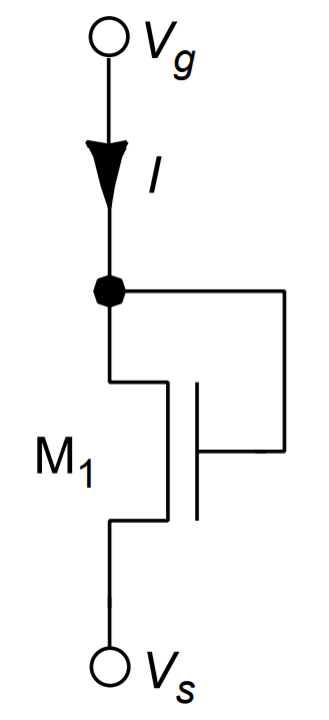
\includegraphics[width=0.15\linewidth]{../../Figures/Diode_Connected_NFET.PNG}
    \caption{Diode Connected nFET. Adapted from Lecture Notes.}
    \label{fig:basalandcerebellum}
\end{figure}

\textbf{Maybe this is confusing?: First, let's remind ourselves that there is an infinite impedance between the channel and the gate. This is because of the physics of transistors, where the gate is separated from the channel with an insulator, which makes the impedance infinite. In simple words, no charge is flowing between the gate and the channel. That also means that you cannot influence the gate charge $V_g$ by the input current.}

Here we connect our circuit to make $V_g = V_d$. If we go from our subthreshold equation:

\begin{equation}
I_{ds} = I_{n0} e^{\frac{\kappa_{n}V_g}{U_T}}(e^\frac{-V_s}{U_T} - e^\frac{-V_d}{U_T})
\end{equation} 

we can rearrange as follows: 

\begin{equation}
I_{ds} = I_{n0} e^{\frac{\kappa_{n}V_g}{U_T}}(e^\frac{-V_s}{U_T} - e^\frac{-V_g}{U_T}) = I_{n0} (e^{\frac{\kappa_{n}V_g - V_s}{U_T}} - e^\frac{\kappa_{n}V_g - V_g}{U_T})
\end{equation}

\begin{equation}
I_{ds} = I_{n0} e^{\frac{\kappa_{n}V_g - V_s}{U_T}} - e^\frac{\kappa_{n}V_g - V_g}{U_T}
\end{equation}

Remember, we love assumptions and simplifications of calculations here. So we keep on assuming that $\kappa_n \approx 1$ and thus reach back the familiar saturation equation:

\begin{equation}
I_{ds} = I_{n0} e^{\frac{\kappa_{n}V_g - V_s}{U_T}}
\end{equation}

So now, when a transistor is diode connected, it actually \emph{is} in saturation, it's not an assumption anymore (well it always kinda is, but less than before :) ). That's also why it's called a diode connected transistor: the transfer function is always exponential, just like a diode. Now the critical thing to understand is that the first thing happening here is current flowing into a transistor (just imagine a current source as described before). The current flowing creates a feedback loop between the drain and the charge where both automatically adapt to match each other and work saturation.
